\chapter{Gamma detection testing}

The purpose of this experiment is to determine the necessary conditions under which the gamma spectroscopy with selected photodiodes can be performed and find out whether the photodiodes are even capable of detecting gamma rays since some of them are not determined for detection of gamma rays. The determination of detection efficiency is precisely done in following chapters for selected photodiodes. 
\par
For the very first test of photodiodes we assembled a spectrometric setup from ORTEC modules including preamplifier ORTEC142A, shaping amplifier 575A and high voltage power supply 556 inside the ORTEC minibin. The pulses were captured by EASY-MCA-2K from ORTEC connected to PC running the MAESTRO Multichannel Analyzer Emulation Software \cite{maestro}. As radiation source we used $^{57}$Co 50 mCi Mössbauer source from 2016. It was also necessary to cover the part with radiation source with lead shielding blocks.


\begin{figure}[H]
 \centering
 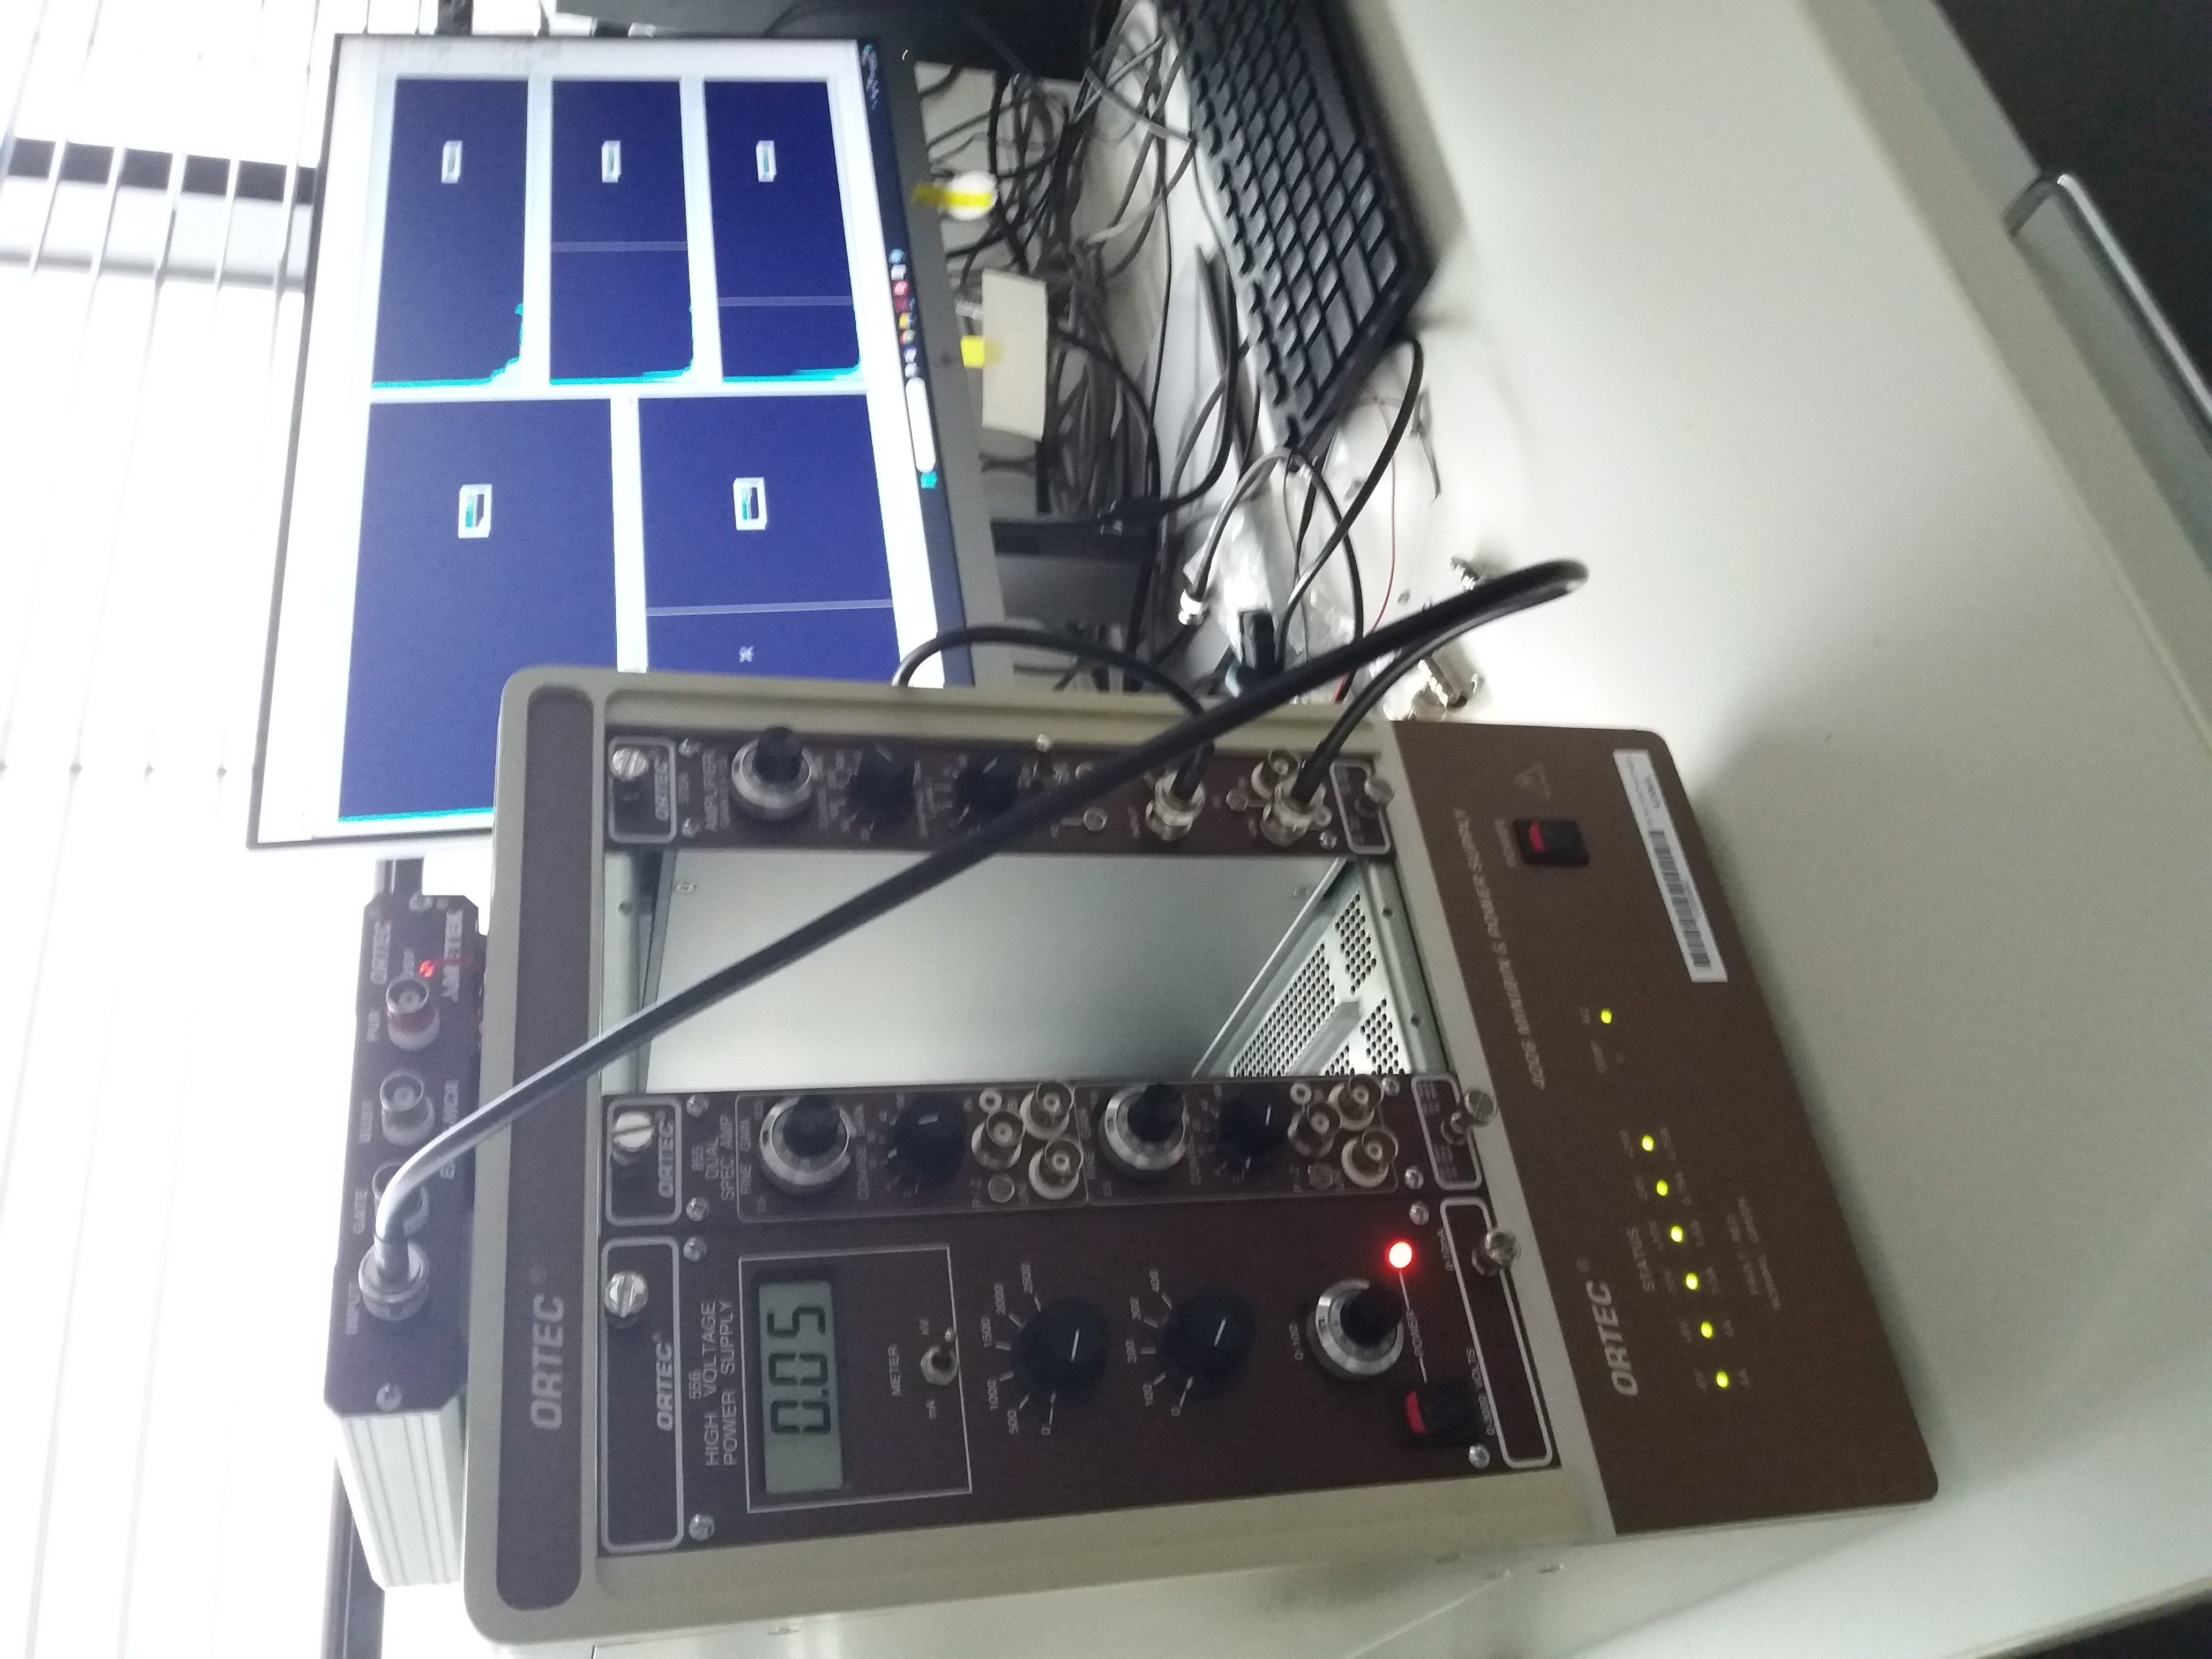
\includegraphics[scale=0.09, angle = 270]{./pictures/ORTECbin.jpg}
 \caption{ORTEC minibin with MCA connected to PC.}
 \label{minibin}
 
\end{figure}




\begin{figure}[H]
 \centering
 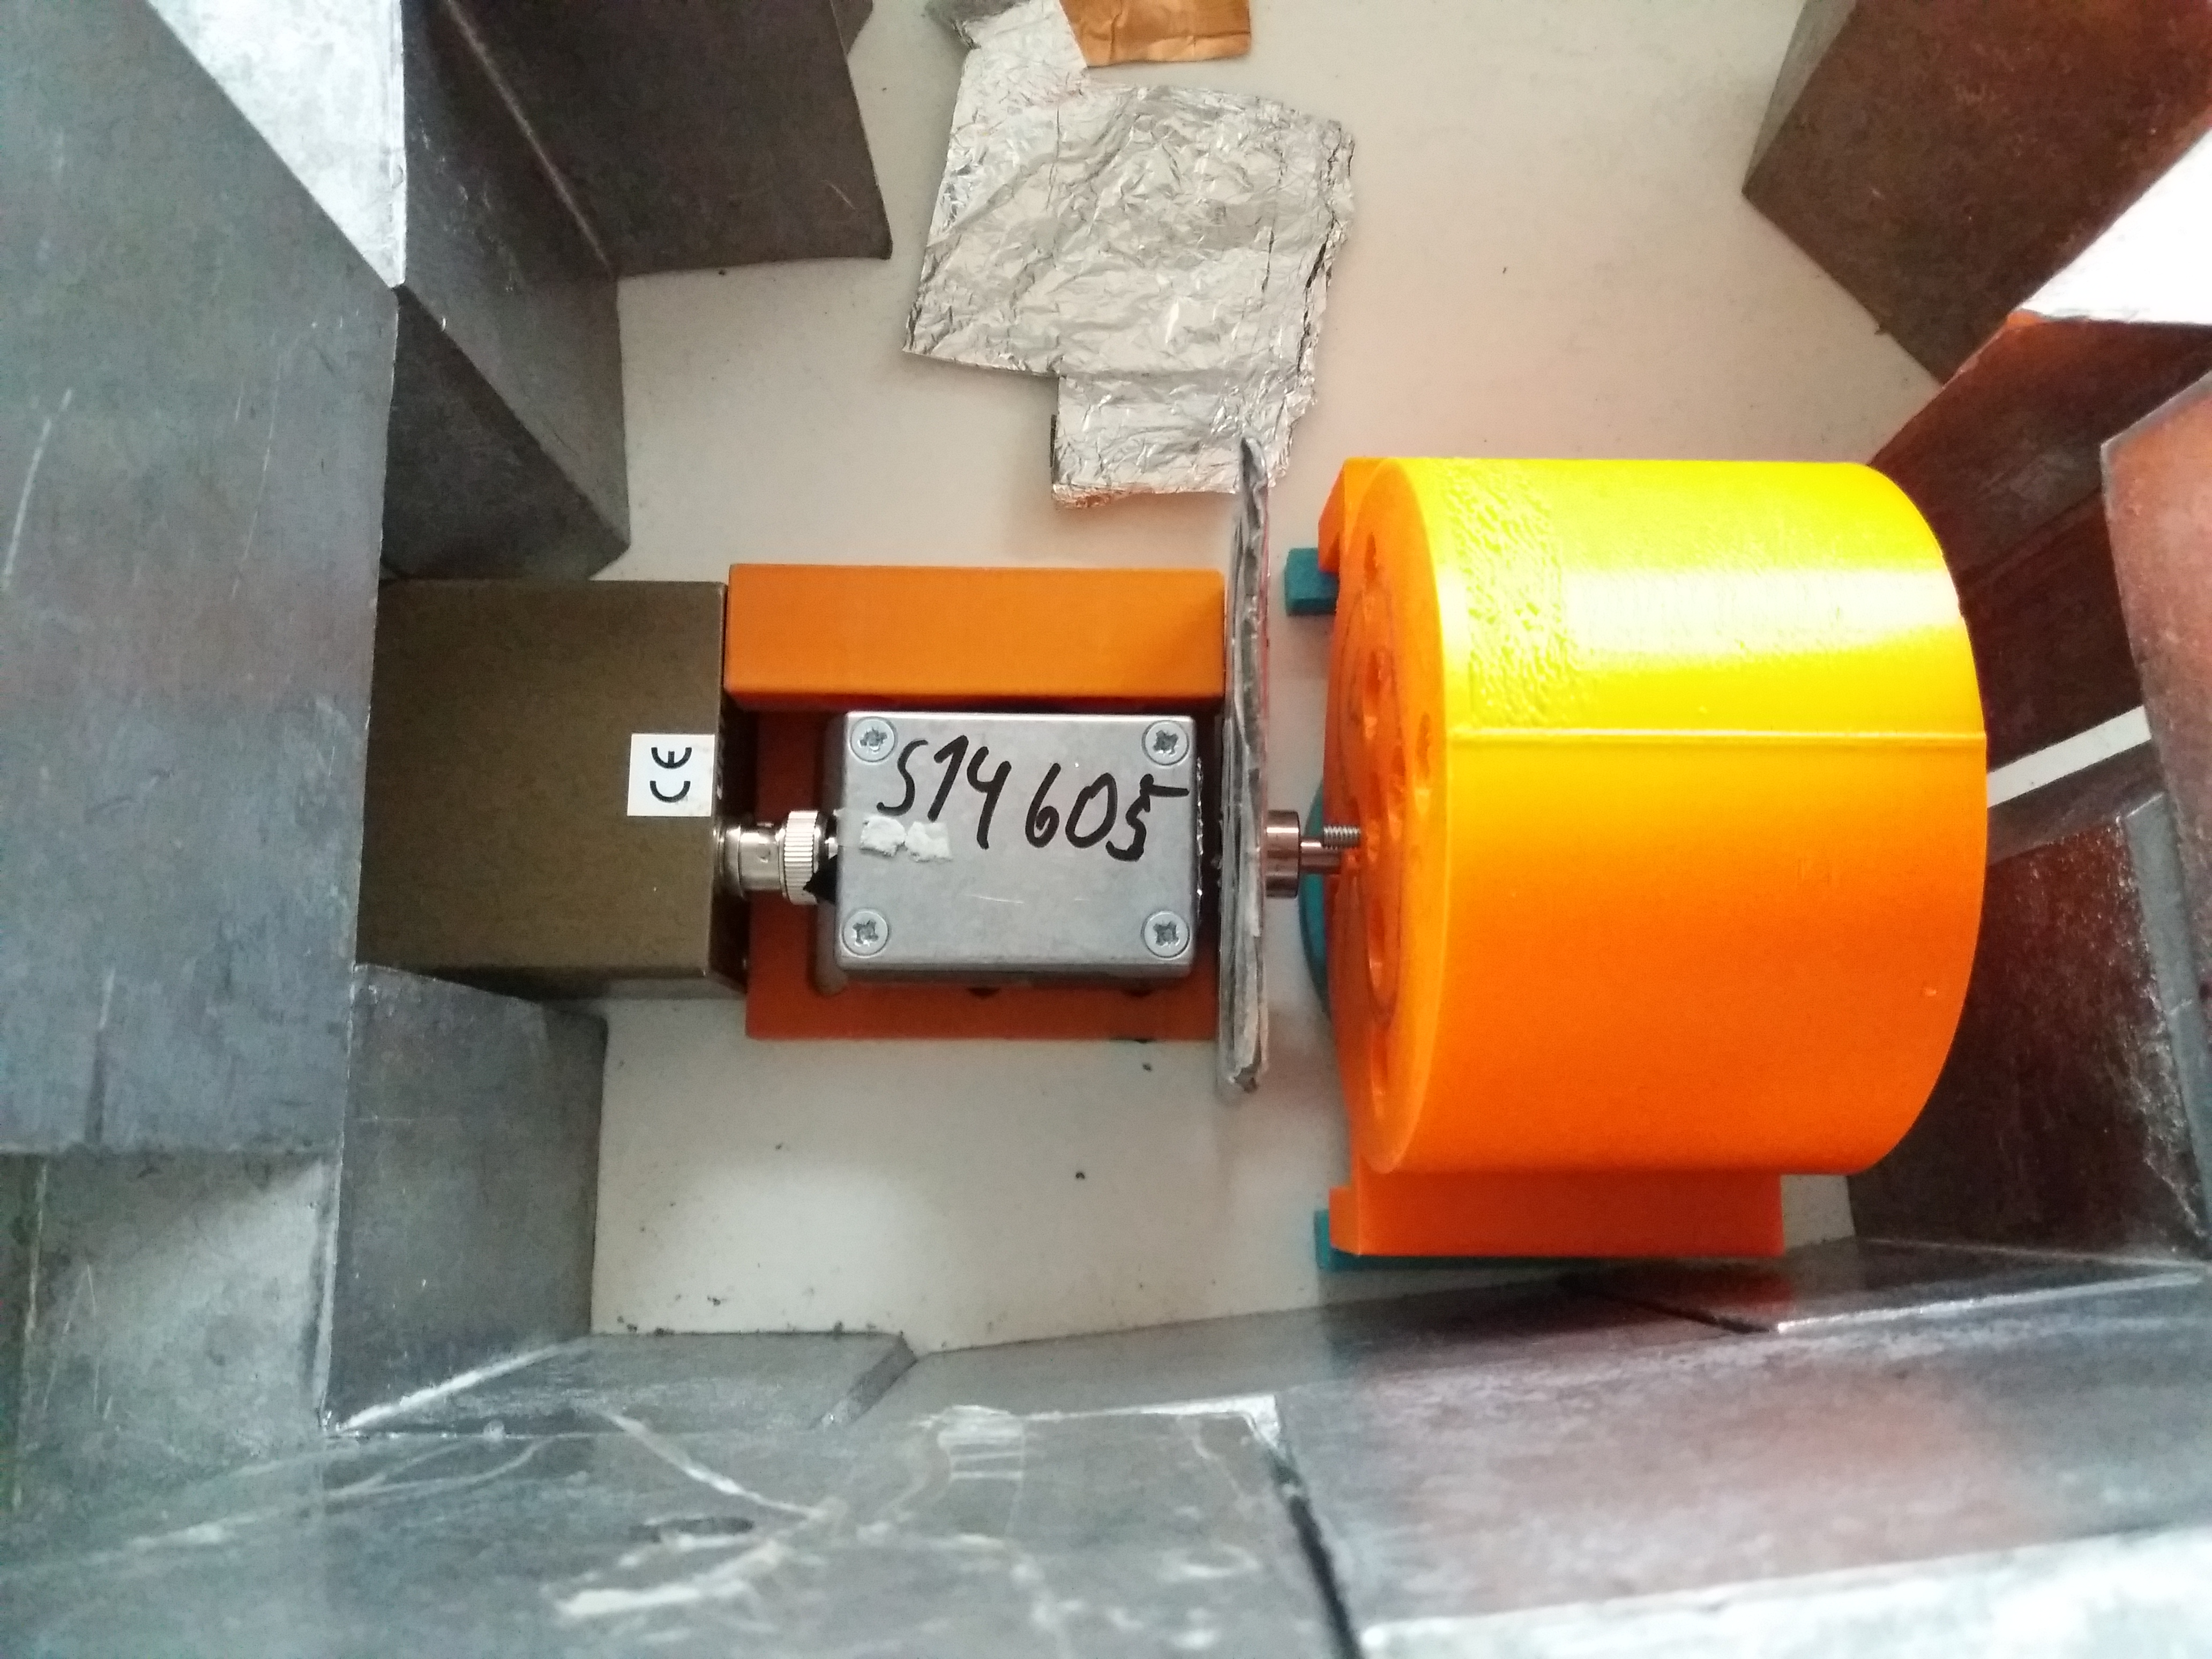
\includegraphics[scale=0.09, angle = 0]{./pictures/ORTECsetup.jpg}
 \caption{PIN diode inside the shielding crate connected to the preamplifier to measure the spectrum of $^{57}$Co source with filter.}
 \label{setup}
 
\end{figure}


\section{Noise and its reduction}
When performing gamma spectroscopy measurements, the energy spectra are affected by noise. In order to reduce noise as much as possible, two approaches were tested - shielding the detector by various ways and cooling to temperatures near 0  $^\circ$C.
\subsection{Electromagnetic noise reduction}
Photodiodes have to be sufficiently electromagnetically shielded and their distance to the preamplifier input should be as short as possible. Using the diodes with poor shielding leads into high levels of electromagnetic noise, which make mayor part of energetic spectra unobservable.
\par
Based on many test it was proven that  the optimal way to shield the photodiode is to put it into the aluminium crate (see Figure \ref{crate}). This crate has to be as small as possible and has to be connected to the grounding potential. However, the front side of the crate has to be open to allow the sufficient transmission of gamma photons to the detector. To preserve the shielding properties, this drilled hole has to be still covered by a conductive material. Our choice was a thin aluminium foil, which has sufficient gamma transmission parameters as well as electromagnetic shielding parameters.

\begin{figure}[H]
 \centering
 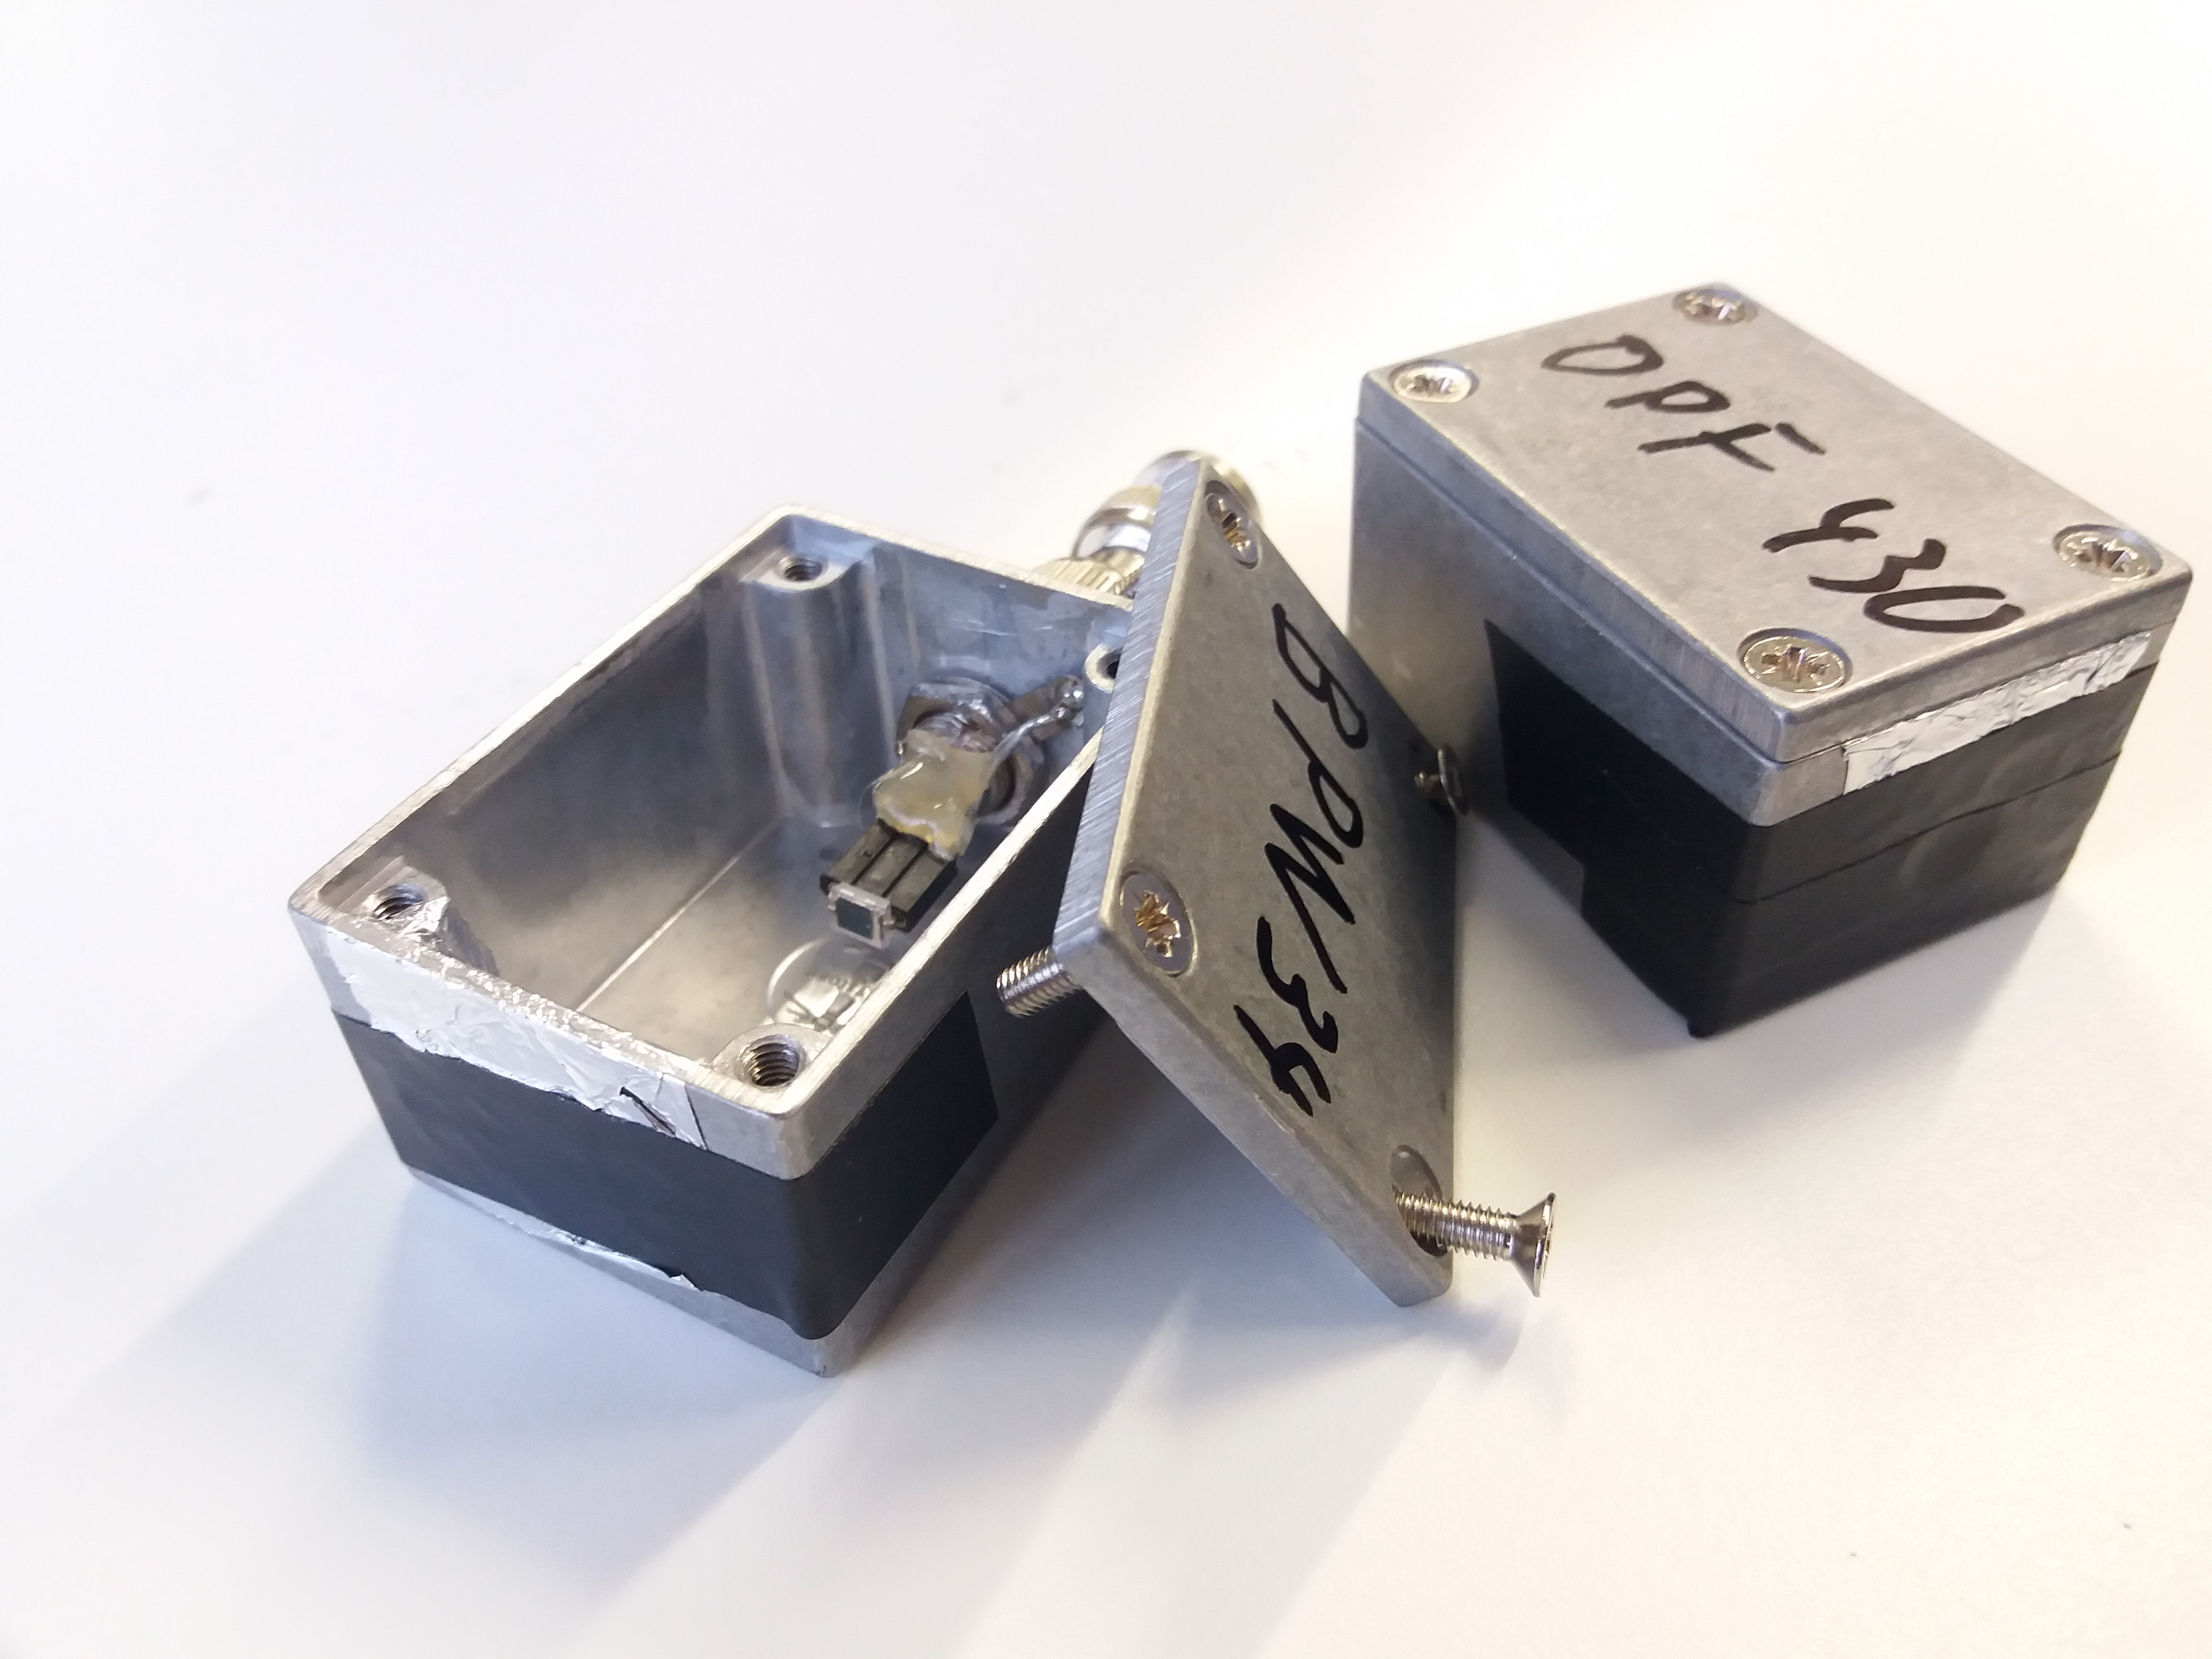
\includegraphics[scale=0.09, angle = 0]{./pictures/ShieldCrate.jpg}
 \caption{Photodiodes inside aluminium shielding crates.}
 \label{crate}
 
\end{figure}


%\begin{figure}[H]
% \centering
% 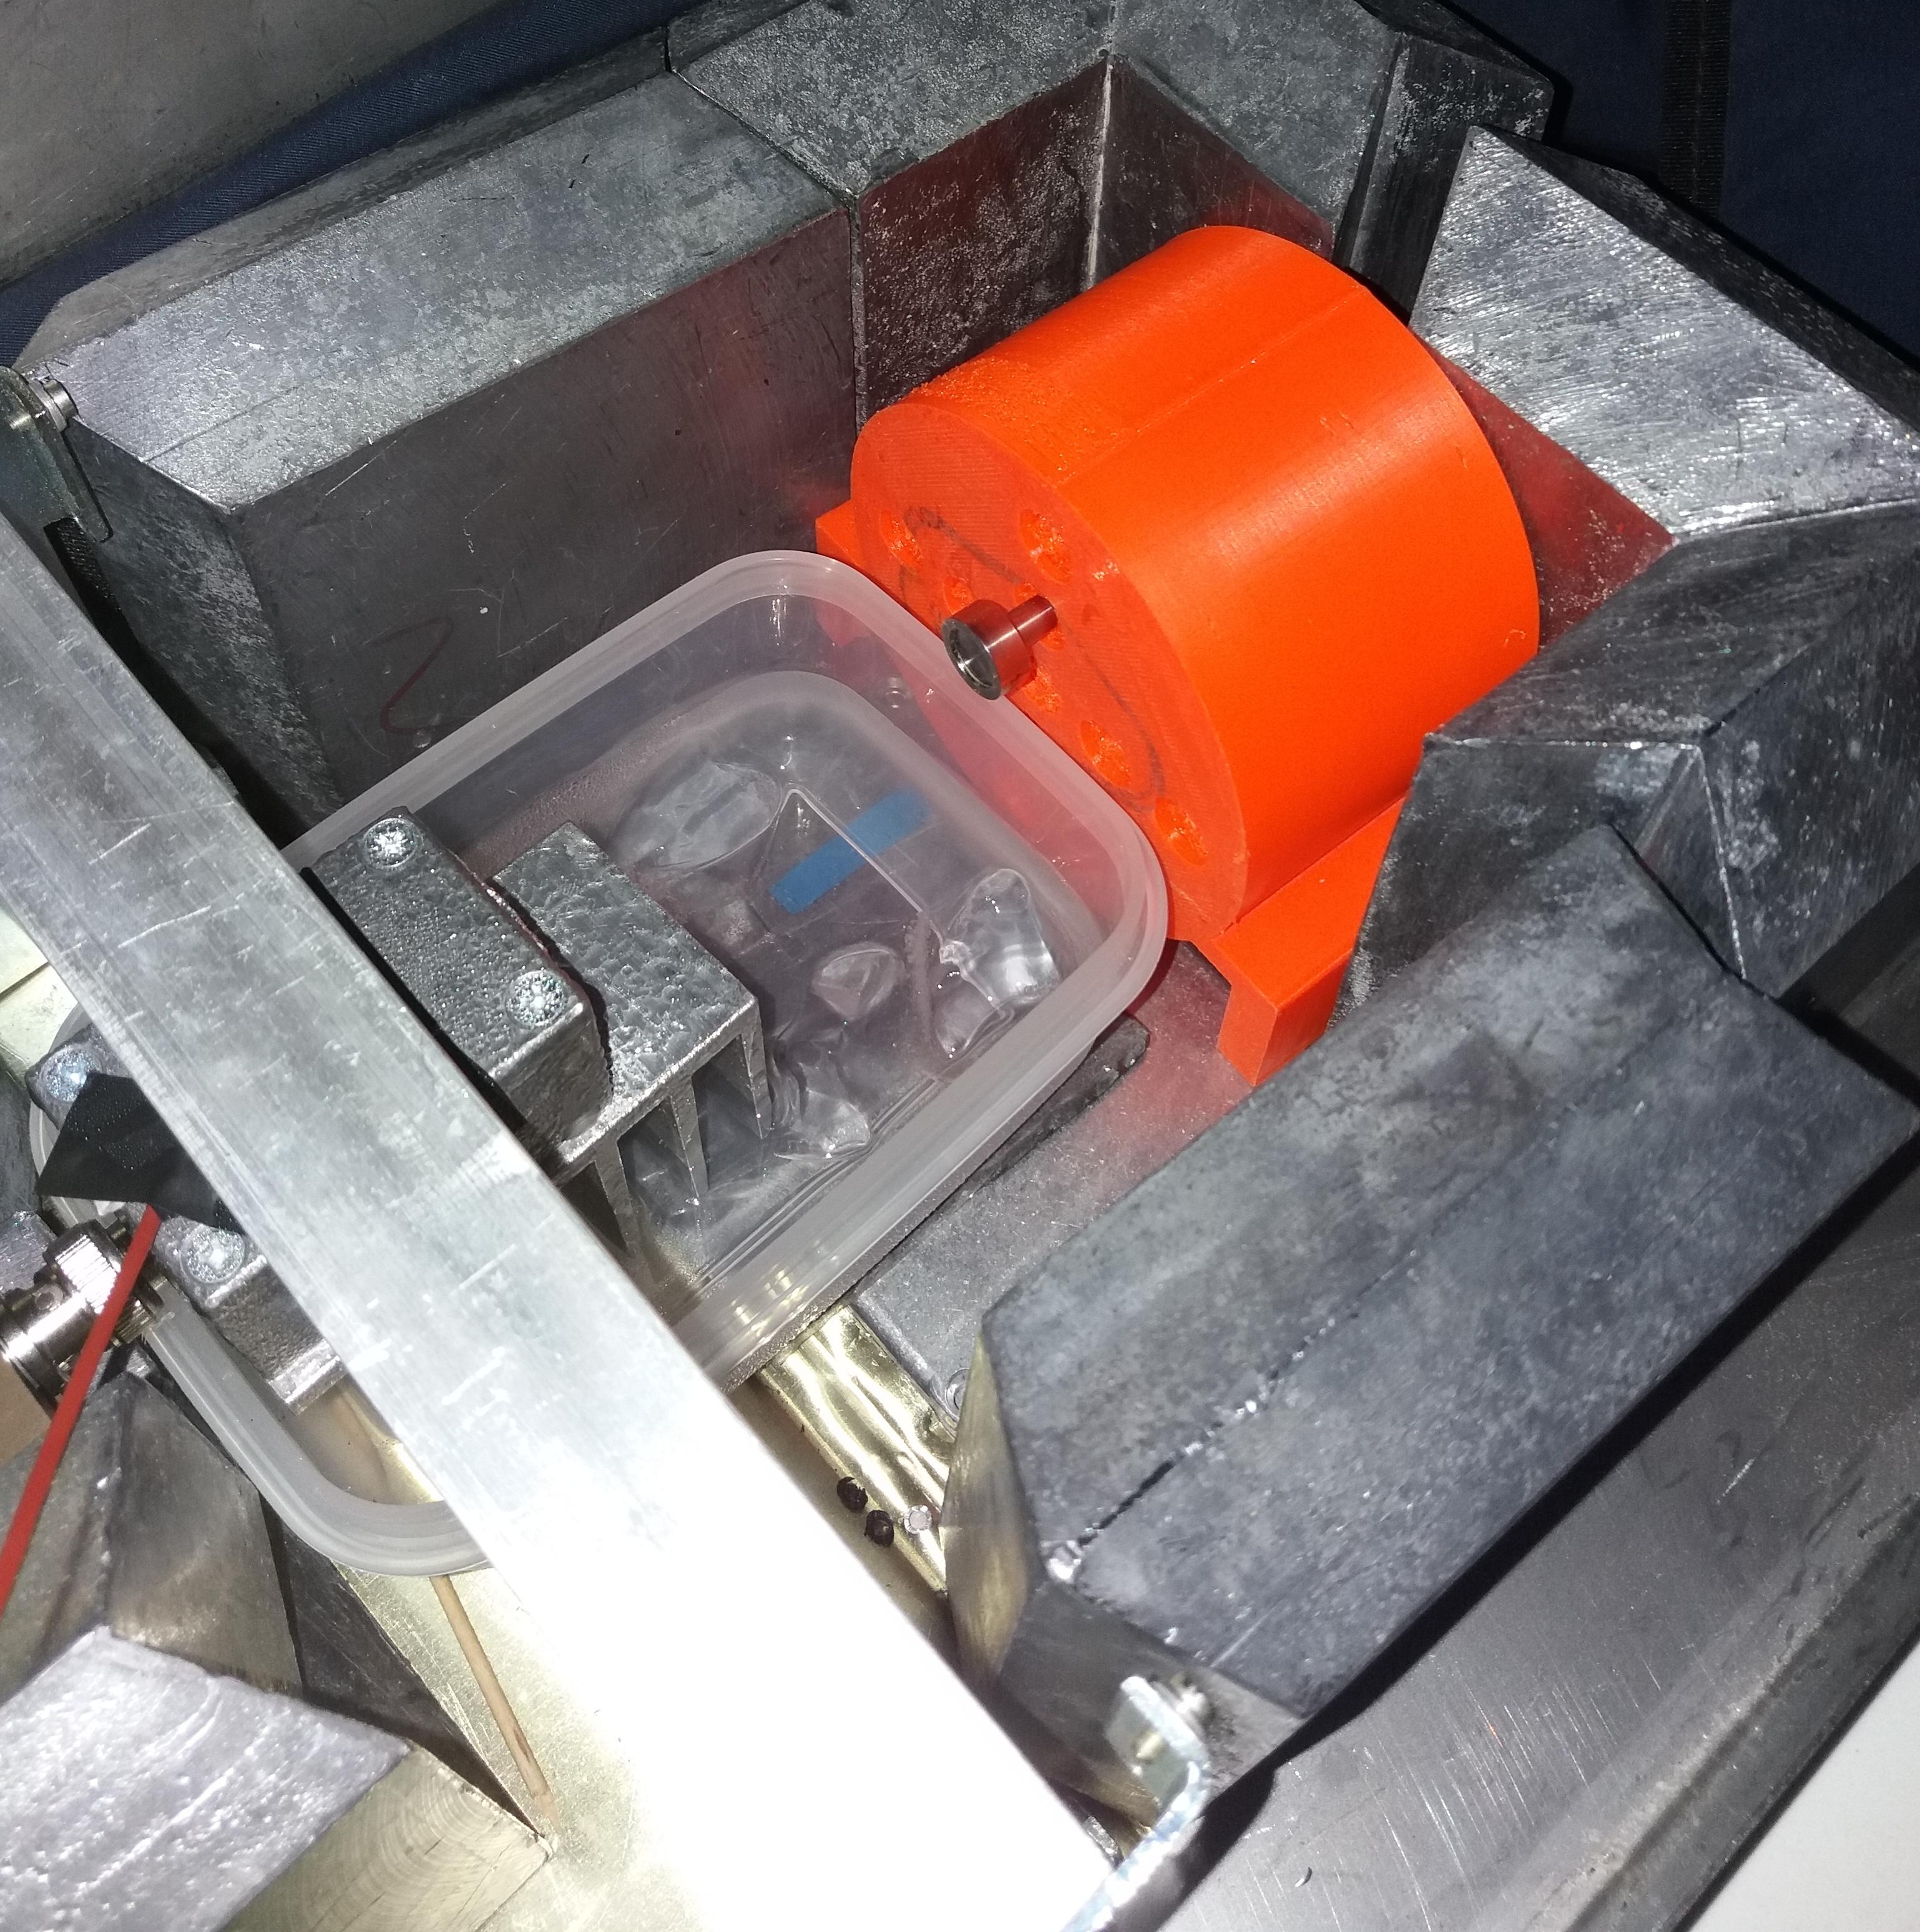
\includegraphics[scale=0.09, angle = 0]{./pictures/chlazeniLedem.jpg}
% \caption{Example of $^{57}$Co spectra from poorly shielded detector setup and from sufficiently shielded detector.}
% \label{notShielded}
% 
%\end{figure}





\subsection{Thermal noise reduction}
To reduce the thermal noise, the S14605 photodiode was cooled by ice. It was placed in shielding box, which had attached heat sink to the bottom. This heat sink was submerged into the small tub filled with an ice (see Figure \ref{cooler}). The thermal conduction was improved by sticking the photodiode to the floor of the shielding box by a conduction paste. The photodiode was cooled this way to temperatures around 7-8 $^\circ$C.


\begin{figure}[H]
 \centering
 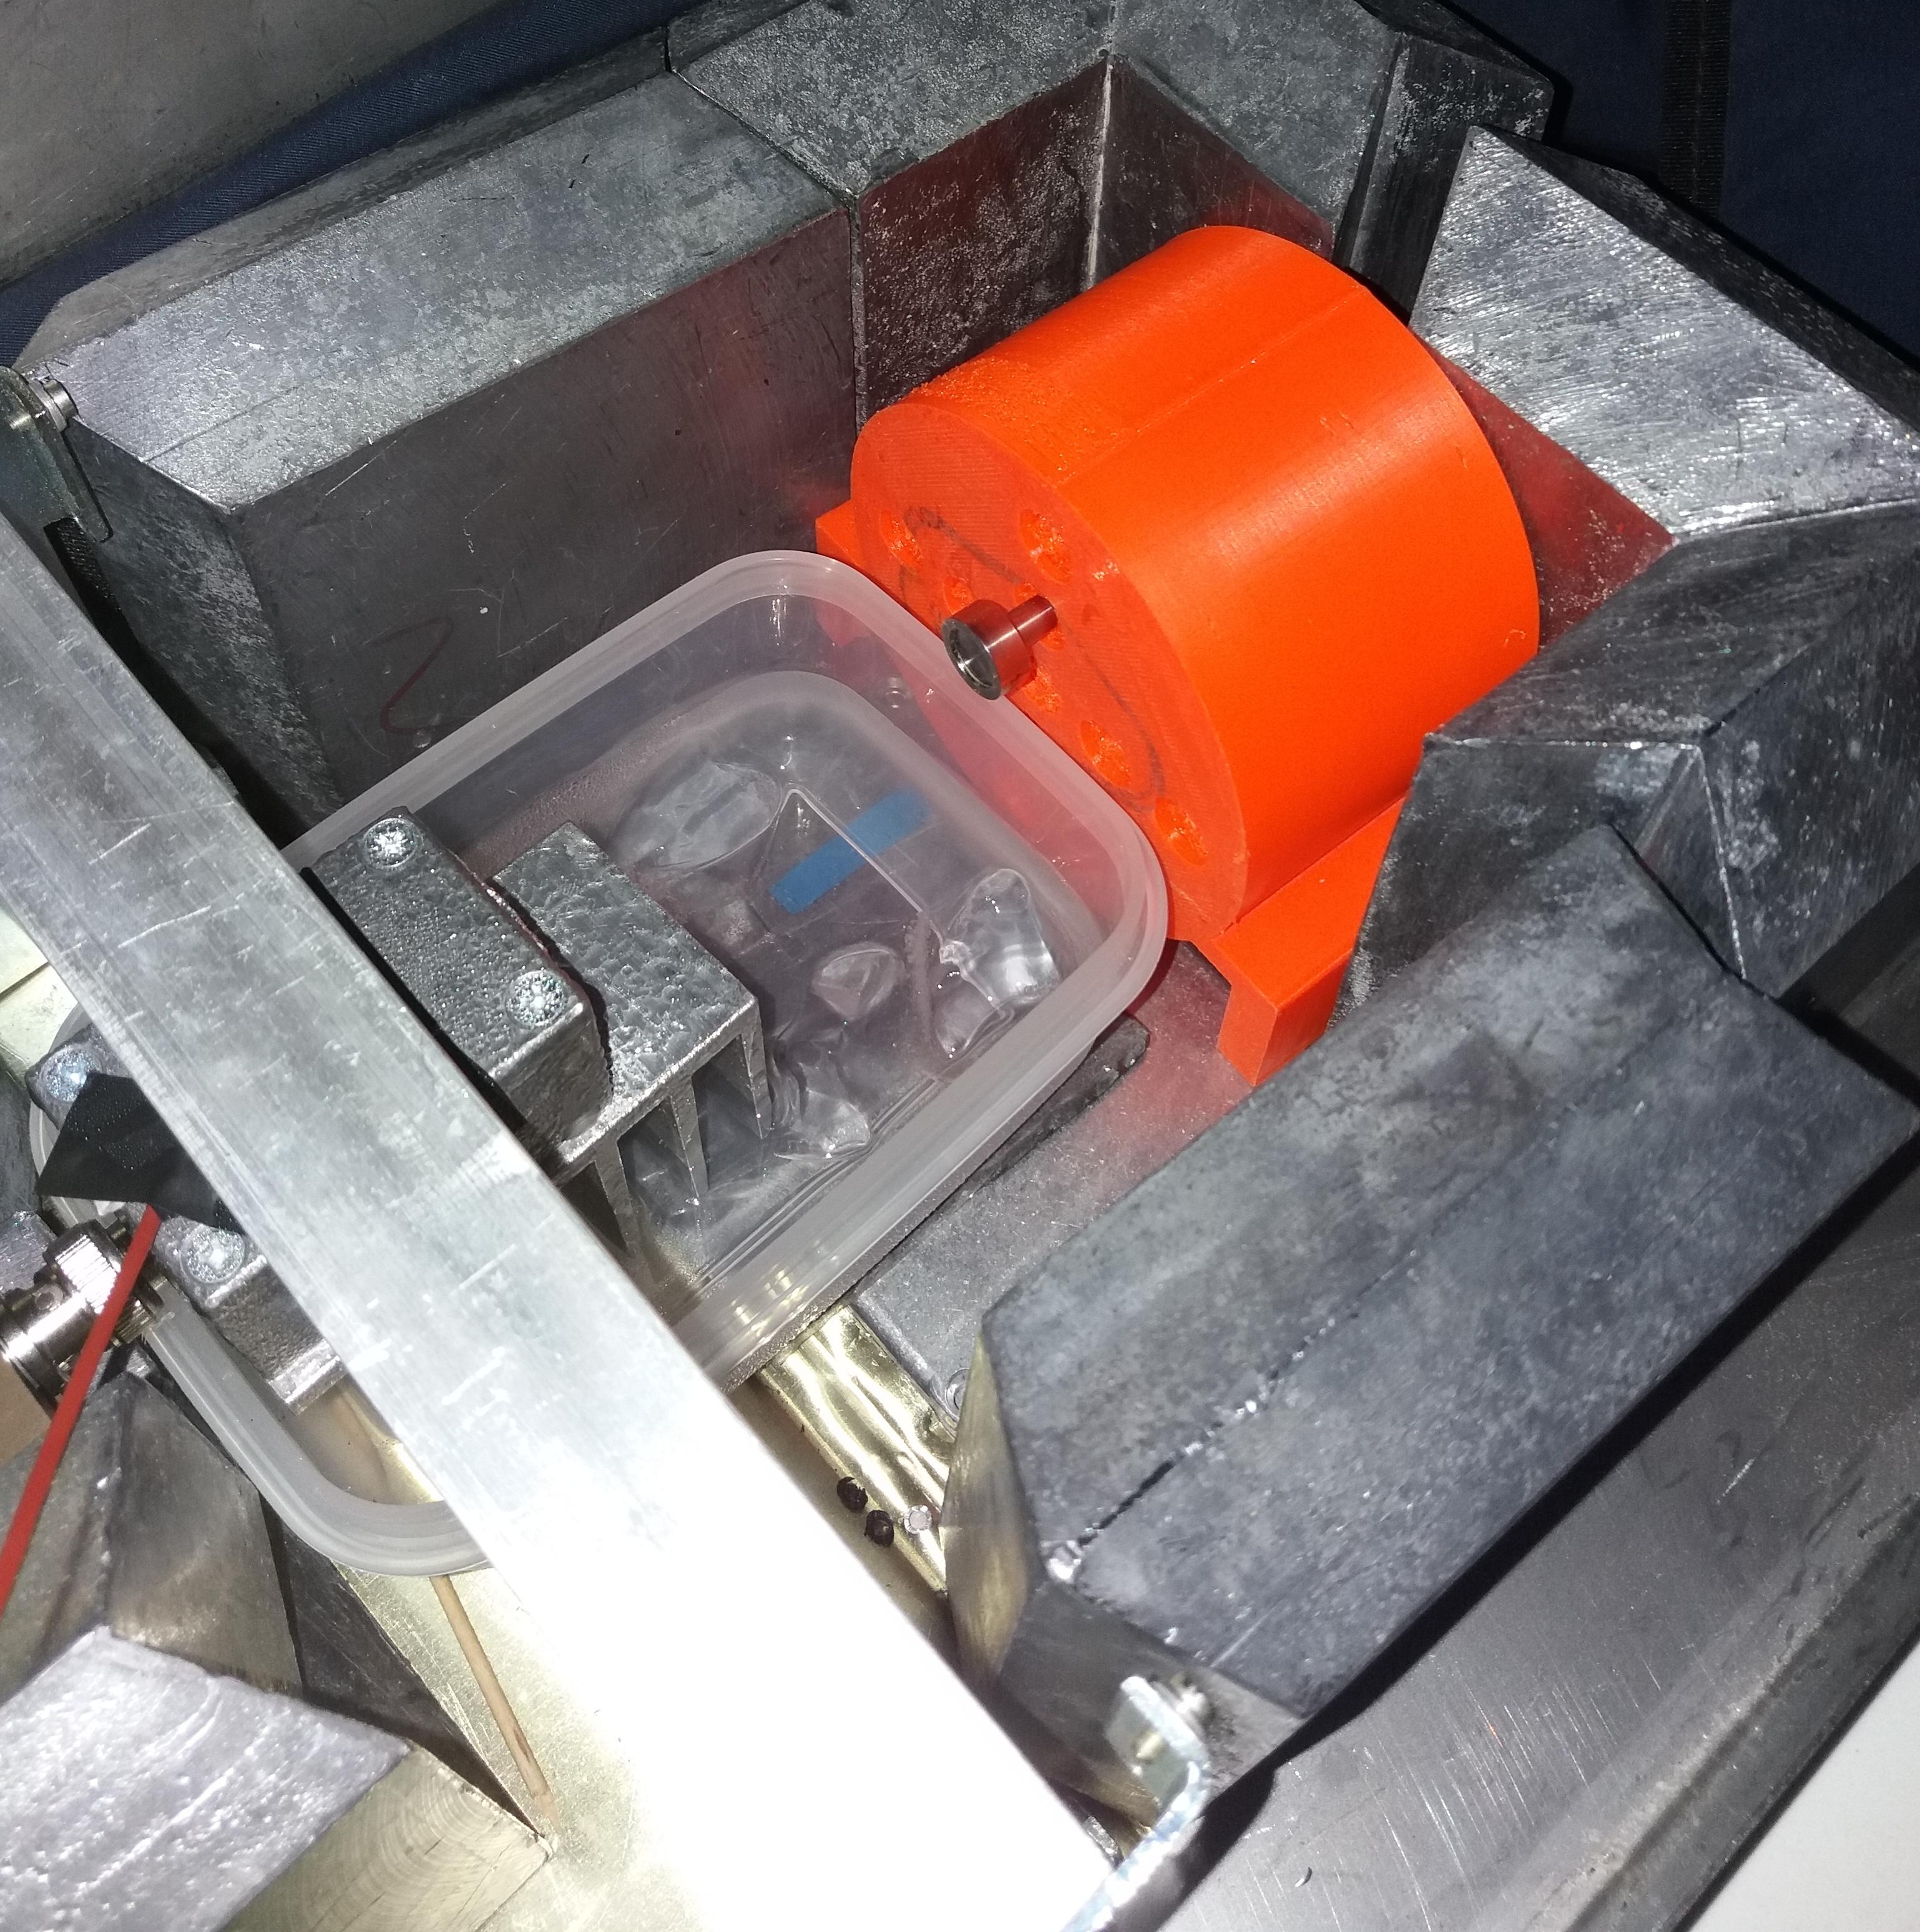
\includegraphics[scale=0.09, angle = 0]{./pictures/chlazeniLedem.jpg}
 \caption{Detector cooled by ice.}
 \label{cooler}
 
\end{figure}



\begin{figure}[H]
 \centering
 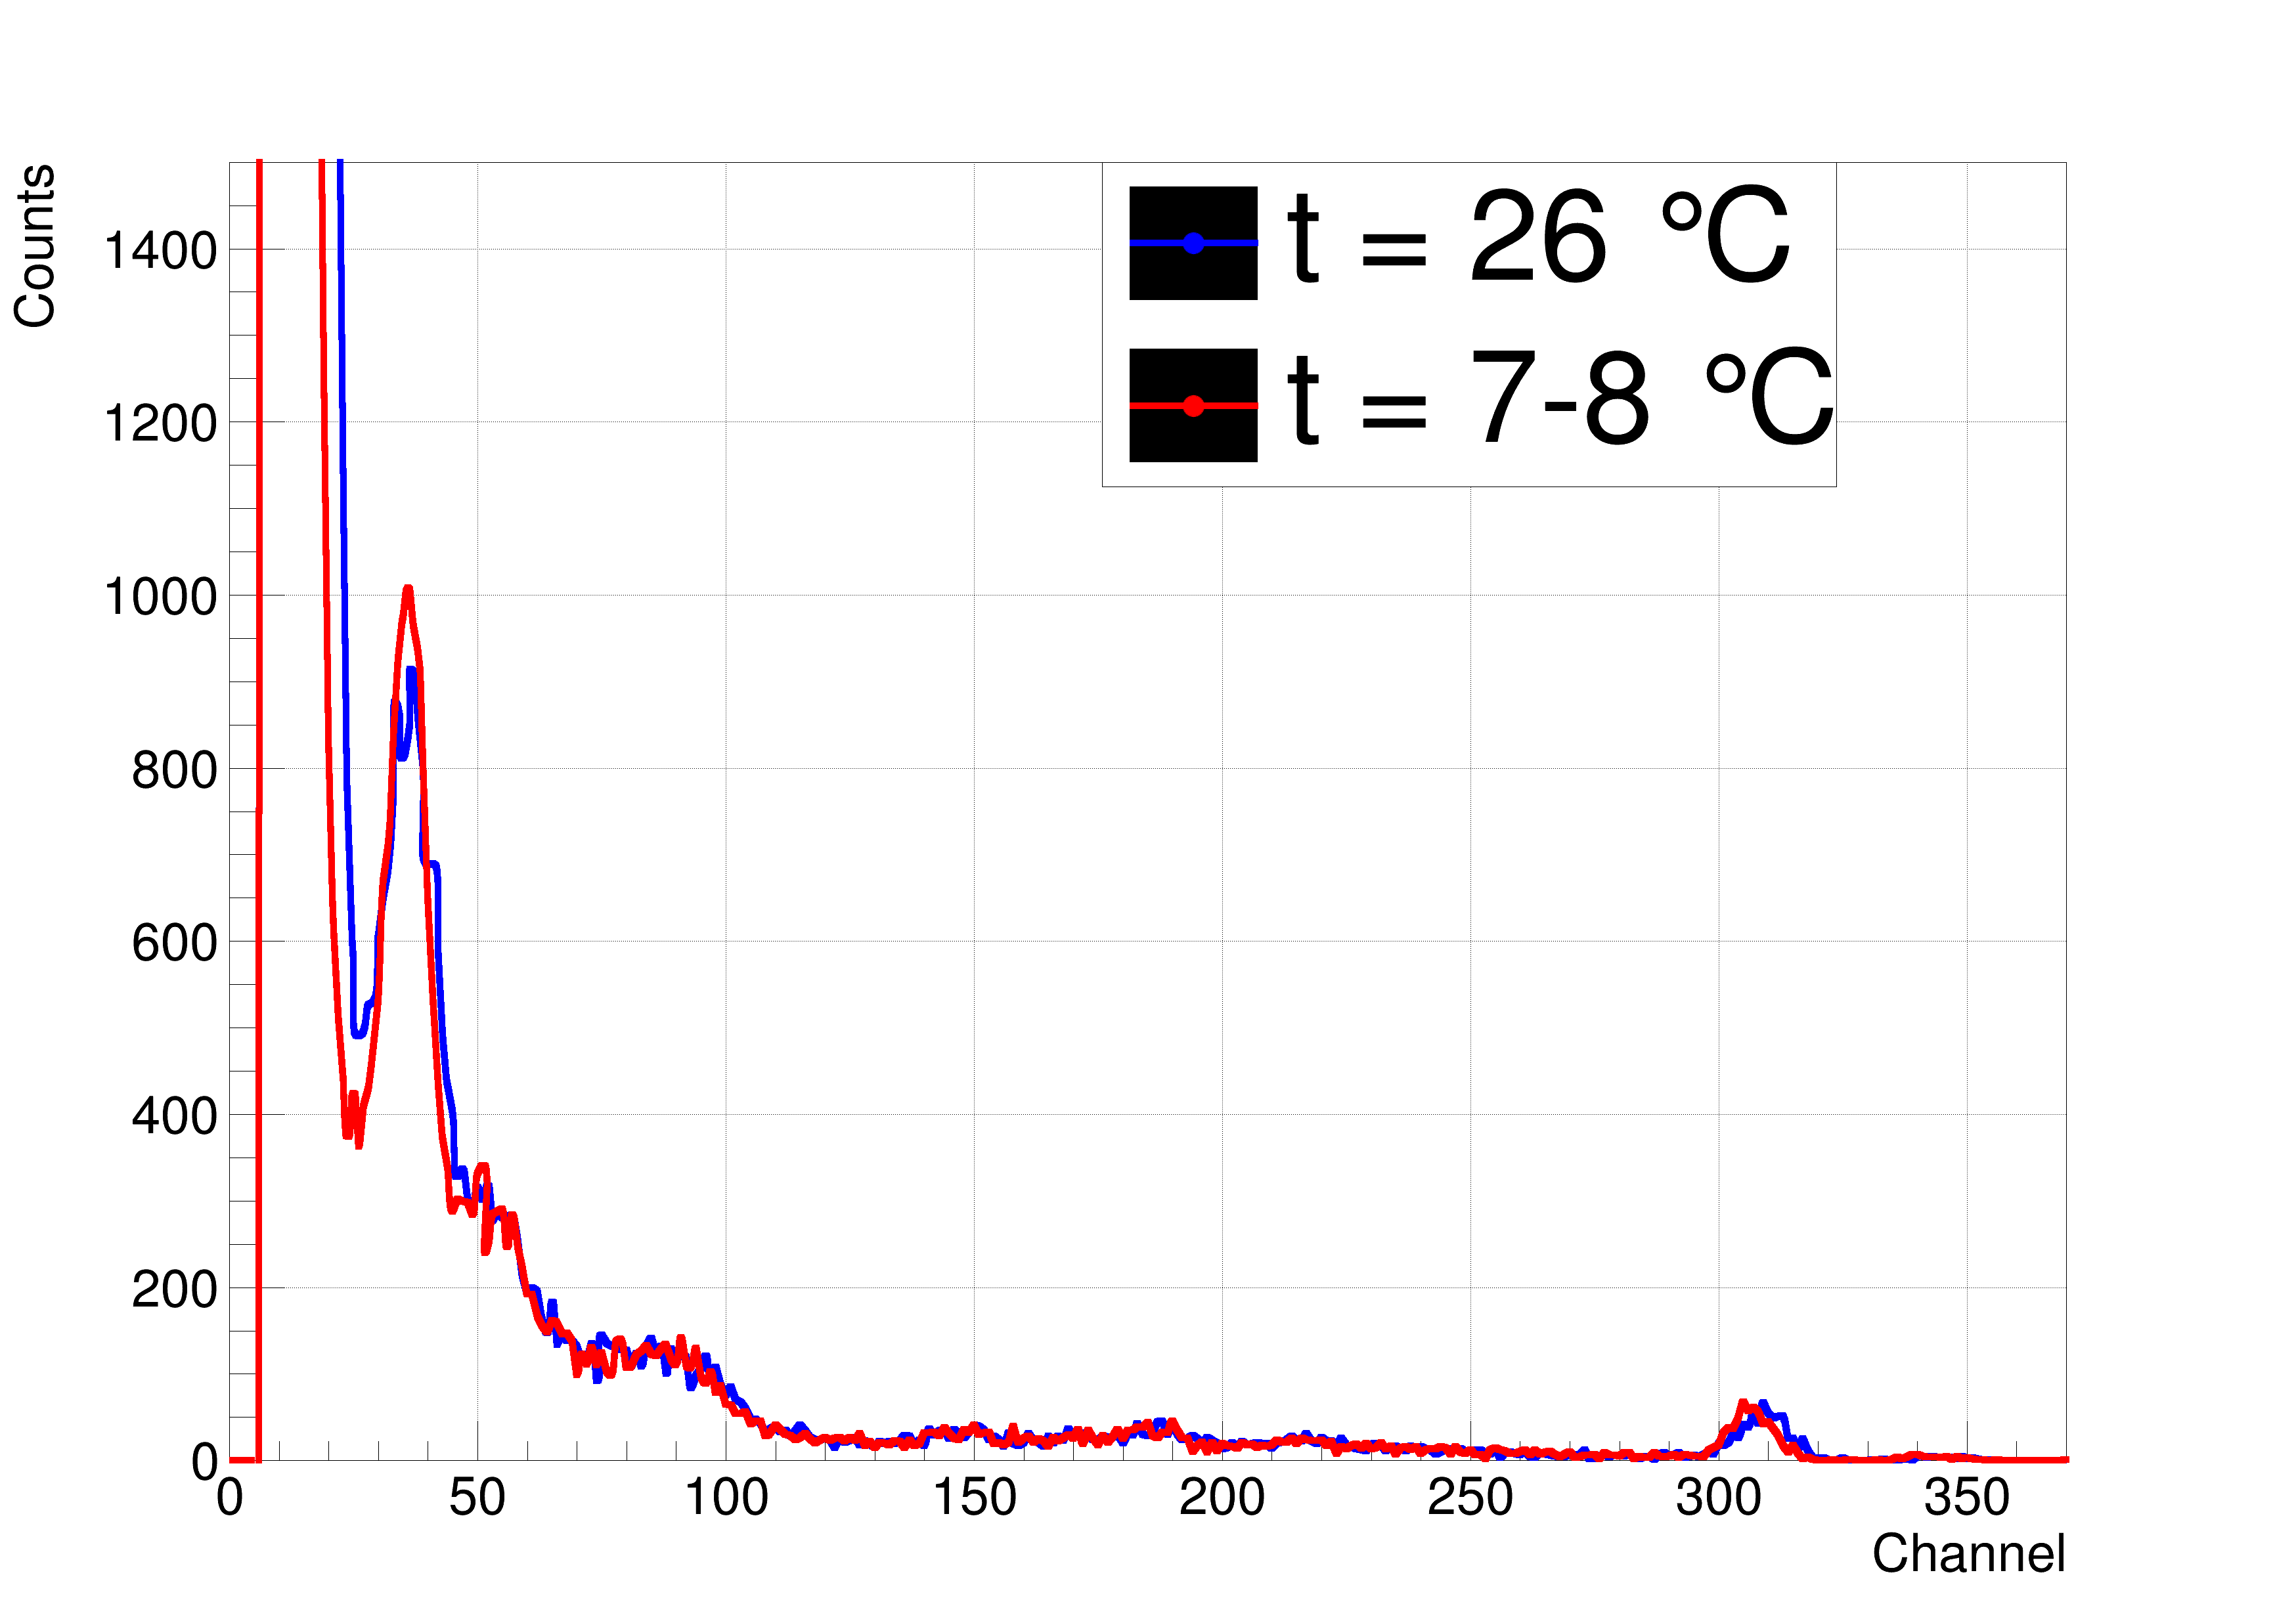
\includegraphics[scale=0.13, angle = 0]{./pictures/TempDiff.png}
 \caption{Measured $^{57}$Co spectra at two different temperatures.}
 \label{coolspectr}
 
\end{figure}








\par
The results show that the cooling improves SNR, but its effect is small when compared to the effect of proper shielding. The cooling is not used in following tests on ORTEC setup.
%It was also tried to use the peltier cooler instead, however, the cooling efficiency was low when compared to the ice.

\section{Detection test of the $^{57}$Co spectra}
The spectra for every photodiode were taken for 30 min of real time (MCA allows dead time compensation) with the source's distance 1 cm from the front shielding crate. There is a simple test with a set of filters, which can help us to find out the corresponding energies to the measured peaks:

\begin{itemize}
\item Pb filter: everything should be attenuated.
\item Cu filter: transmitted - 122.1 keV, 136.5 keV not transmitted - 14.4 keV, 6.4 keV.
\item Al filter: transmitted - 122.1 keV, 136.5 keV, 14.4 keV not transmitted - 6.4 keV.
\end{itemize}

The analysed spectrum is analysed by our peak finder program (described in section \ref{search}) to find the characteristic energy components. By filter test it can be determined which peak corresponds to 14.4 keV (Cu - attenuated, Al - not attenuated). The channel position of 14.4 keV is then used to to calibrate the energy axis of the MCA spectrum.
\par
The Compton edge caused by interaction of 122.1 keV photons inside the detector can be expected. The equation \ref{compton} estimates the position to be around 39.5 keV. 

\subsection{S14605 test}
From the S14605 capacity and dark current graphs (data-sheet \ref{datS14605}) can be deduced optimal voltage. We decided to set it to 50 V, because any further increase of voltage does not improve the SNR. The measured spectra with no filter, with particular filters and only background (fully shielded) are in the Fig. \ref{S14605 spectra}.


\begin{figure}[H]
 \centering
 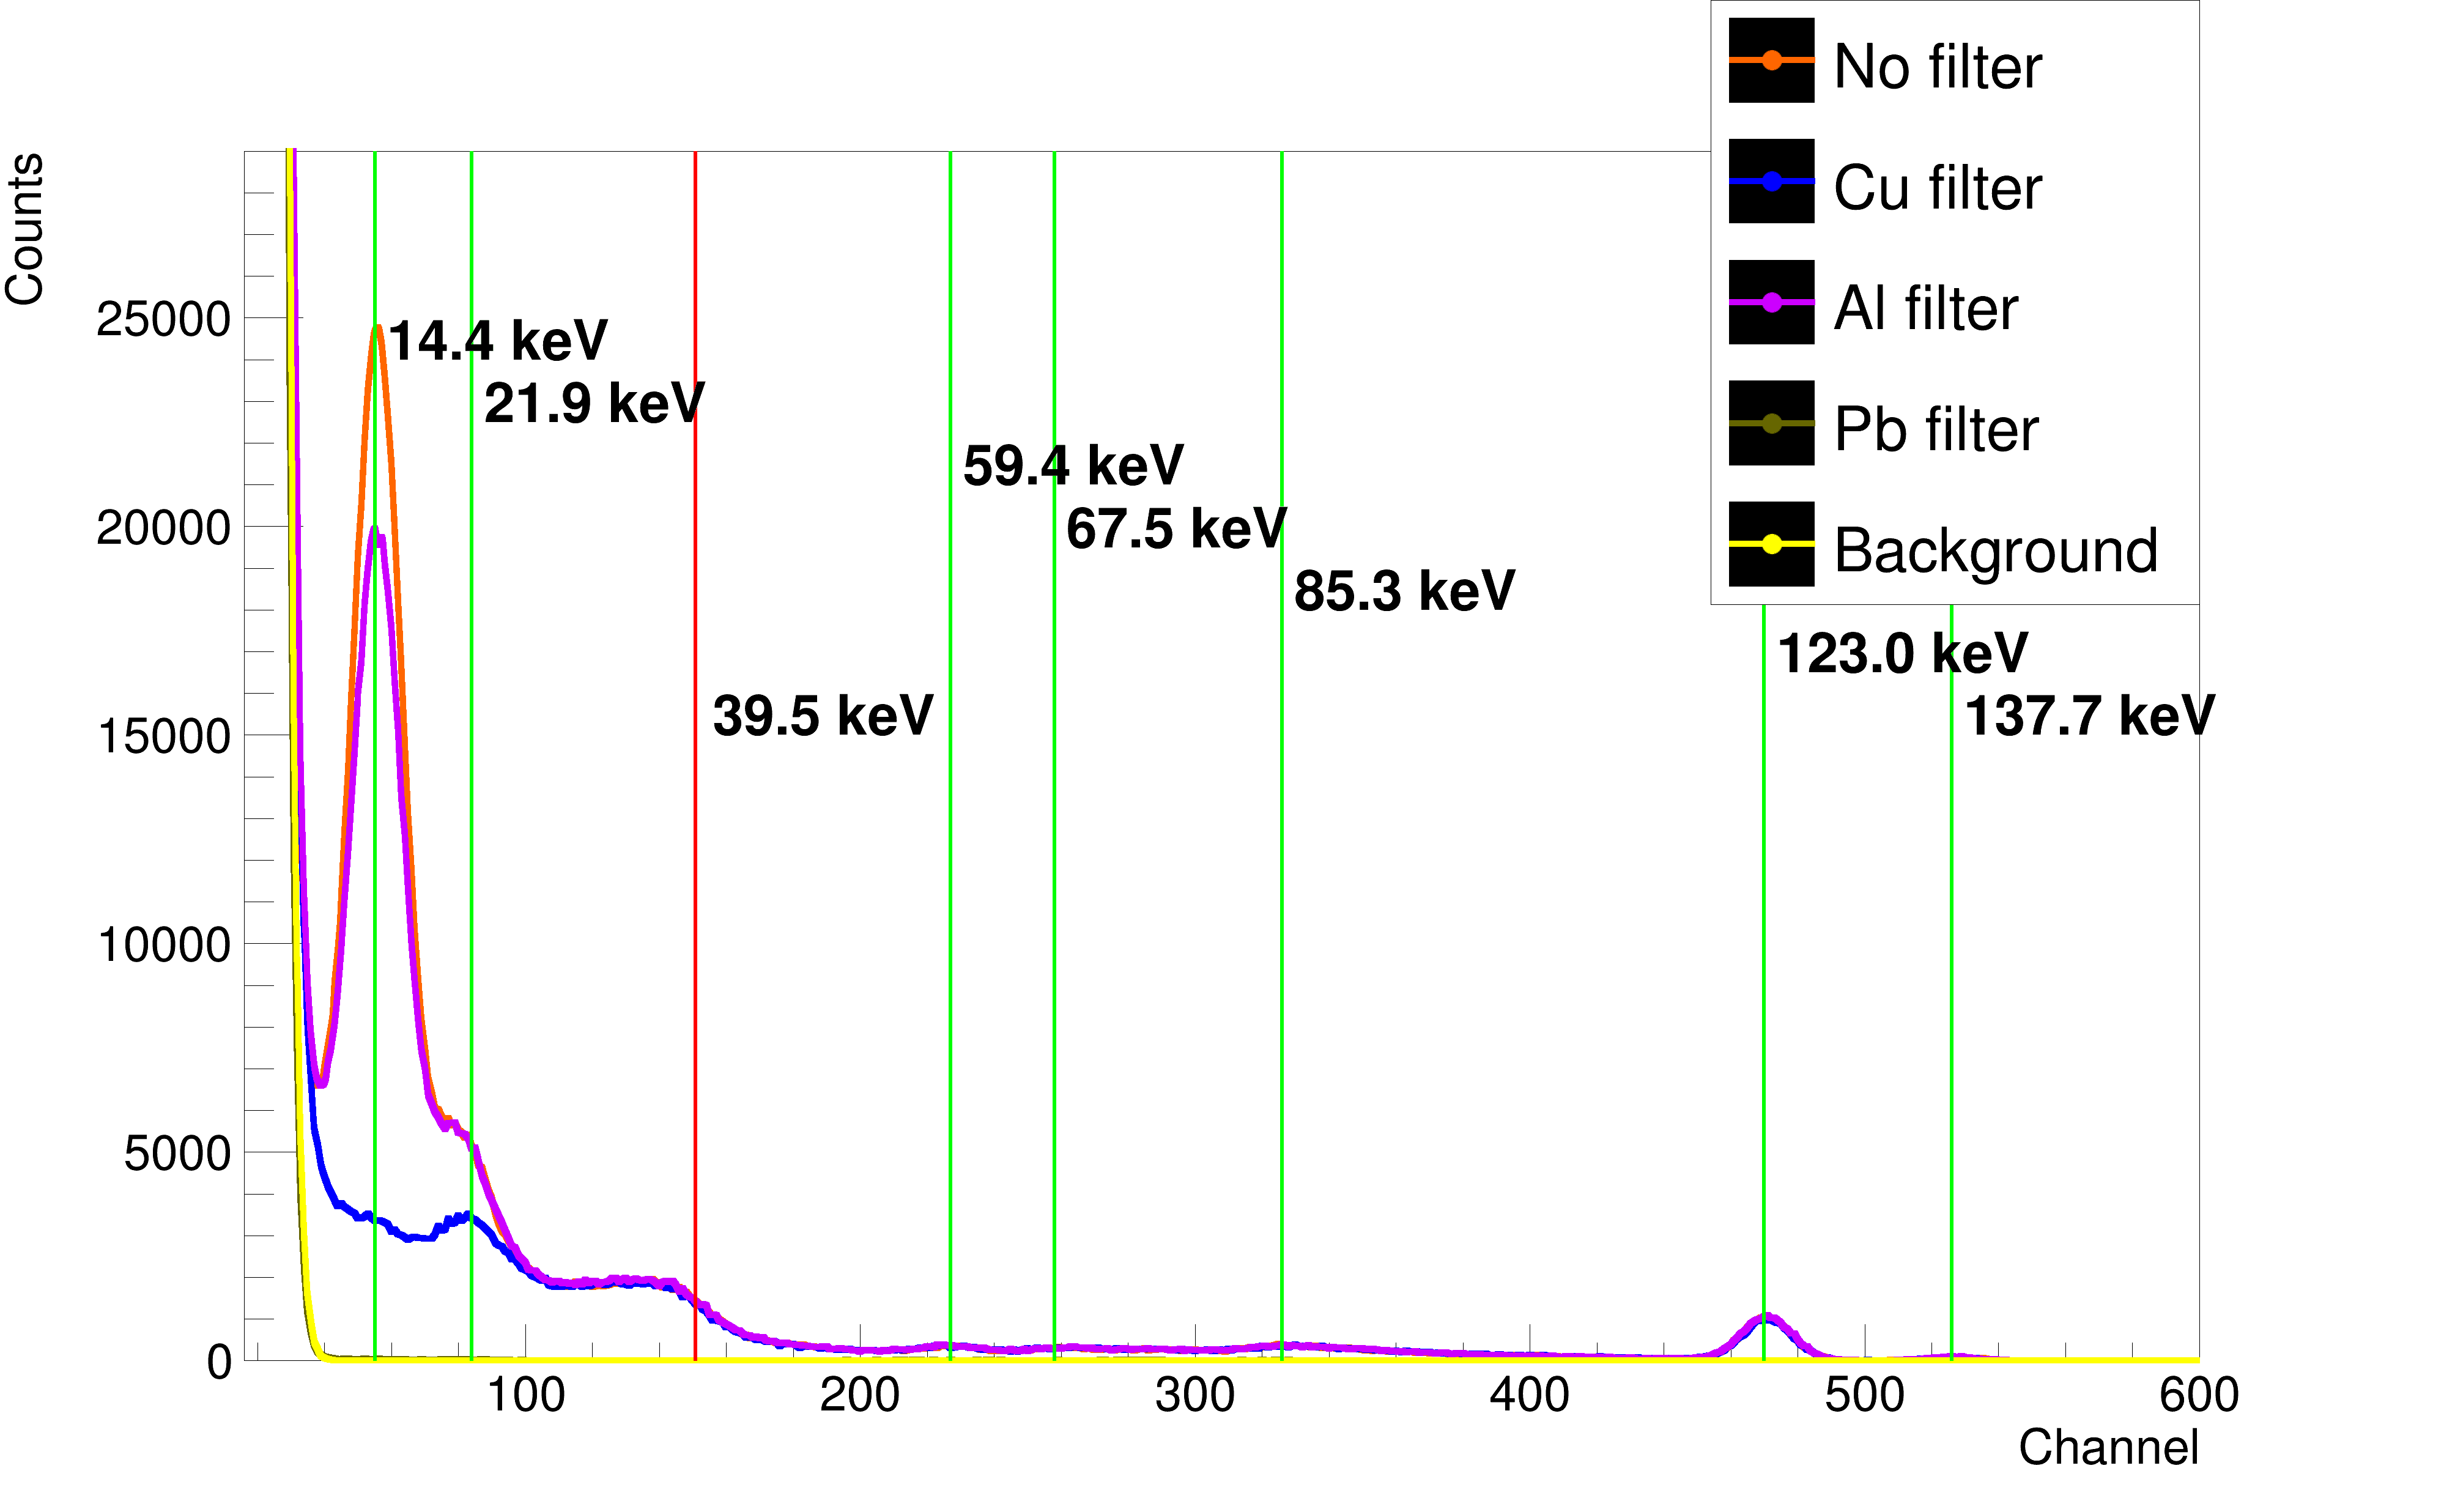
\includegraphics[scale=0.125, angle = 0]{./pictures/S14GammaTest.png}
 \caption{S14605 spectra with founded energy peaks (green lines) and estimated Compton edge (red line).}
 \label{S14605 spectra}
 
\end{figure}


\par

Due to the first peak's attenuation by mentioned filters, this peak is determined as 14.4 keV full energy peak. The 21.9 keV peak originates from characteristic x-rays of rhodium matrice. 59.4 and 67.5 keV 85.3 keV is characteristic x-rays of lead shielding. The last two peaks (123.0 keV, 137.7 keV) are from $^{57}$Co. It can be seen that the full energy detection efficiency of higher energies (122.1 keV) is very small and that the Compton scattering is preferred interaction effect inside detector at these energies, which results into expected Compton edge. The expected peak of 6.4 keV hidden in the electronic noise. The modular ORTEC setup do not allows any further upgrades, so the only way to improve SNR is to integrate the spectrometric chain into PCB. 

\subsection{BPW34 test}
The instrumentation was similar as before, but BPW34 had to be operated at lower bias voltage and thus 20 V was chosen as an optimum.

\begin{figure}[H]
 \centering
 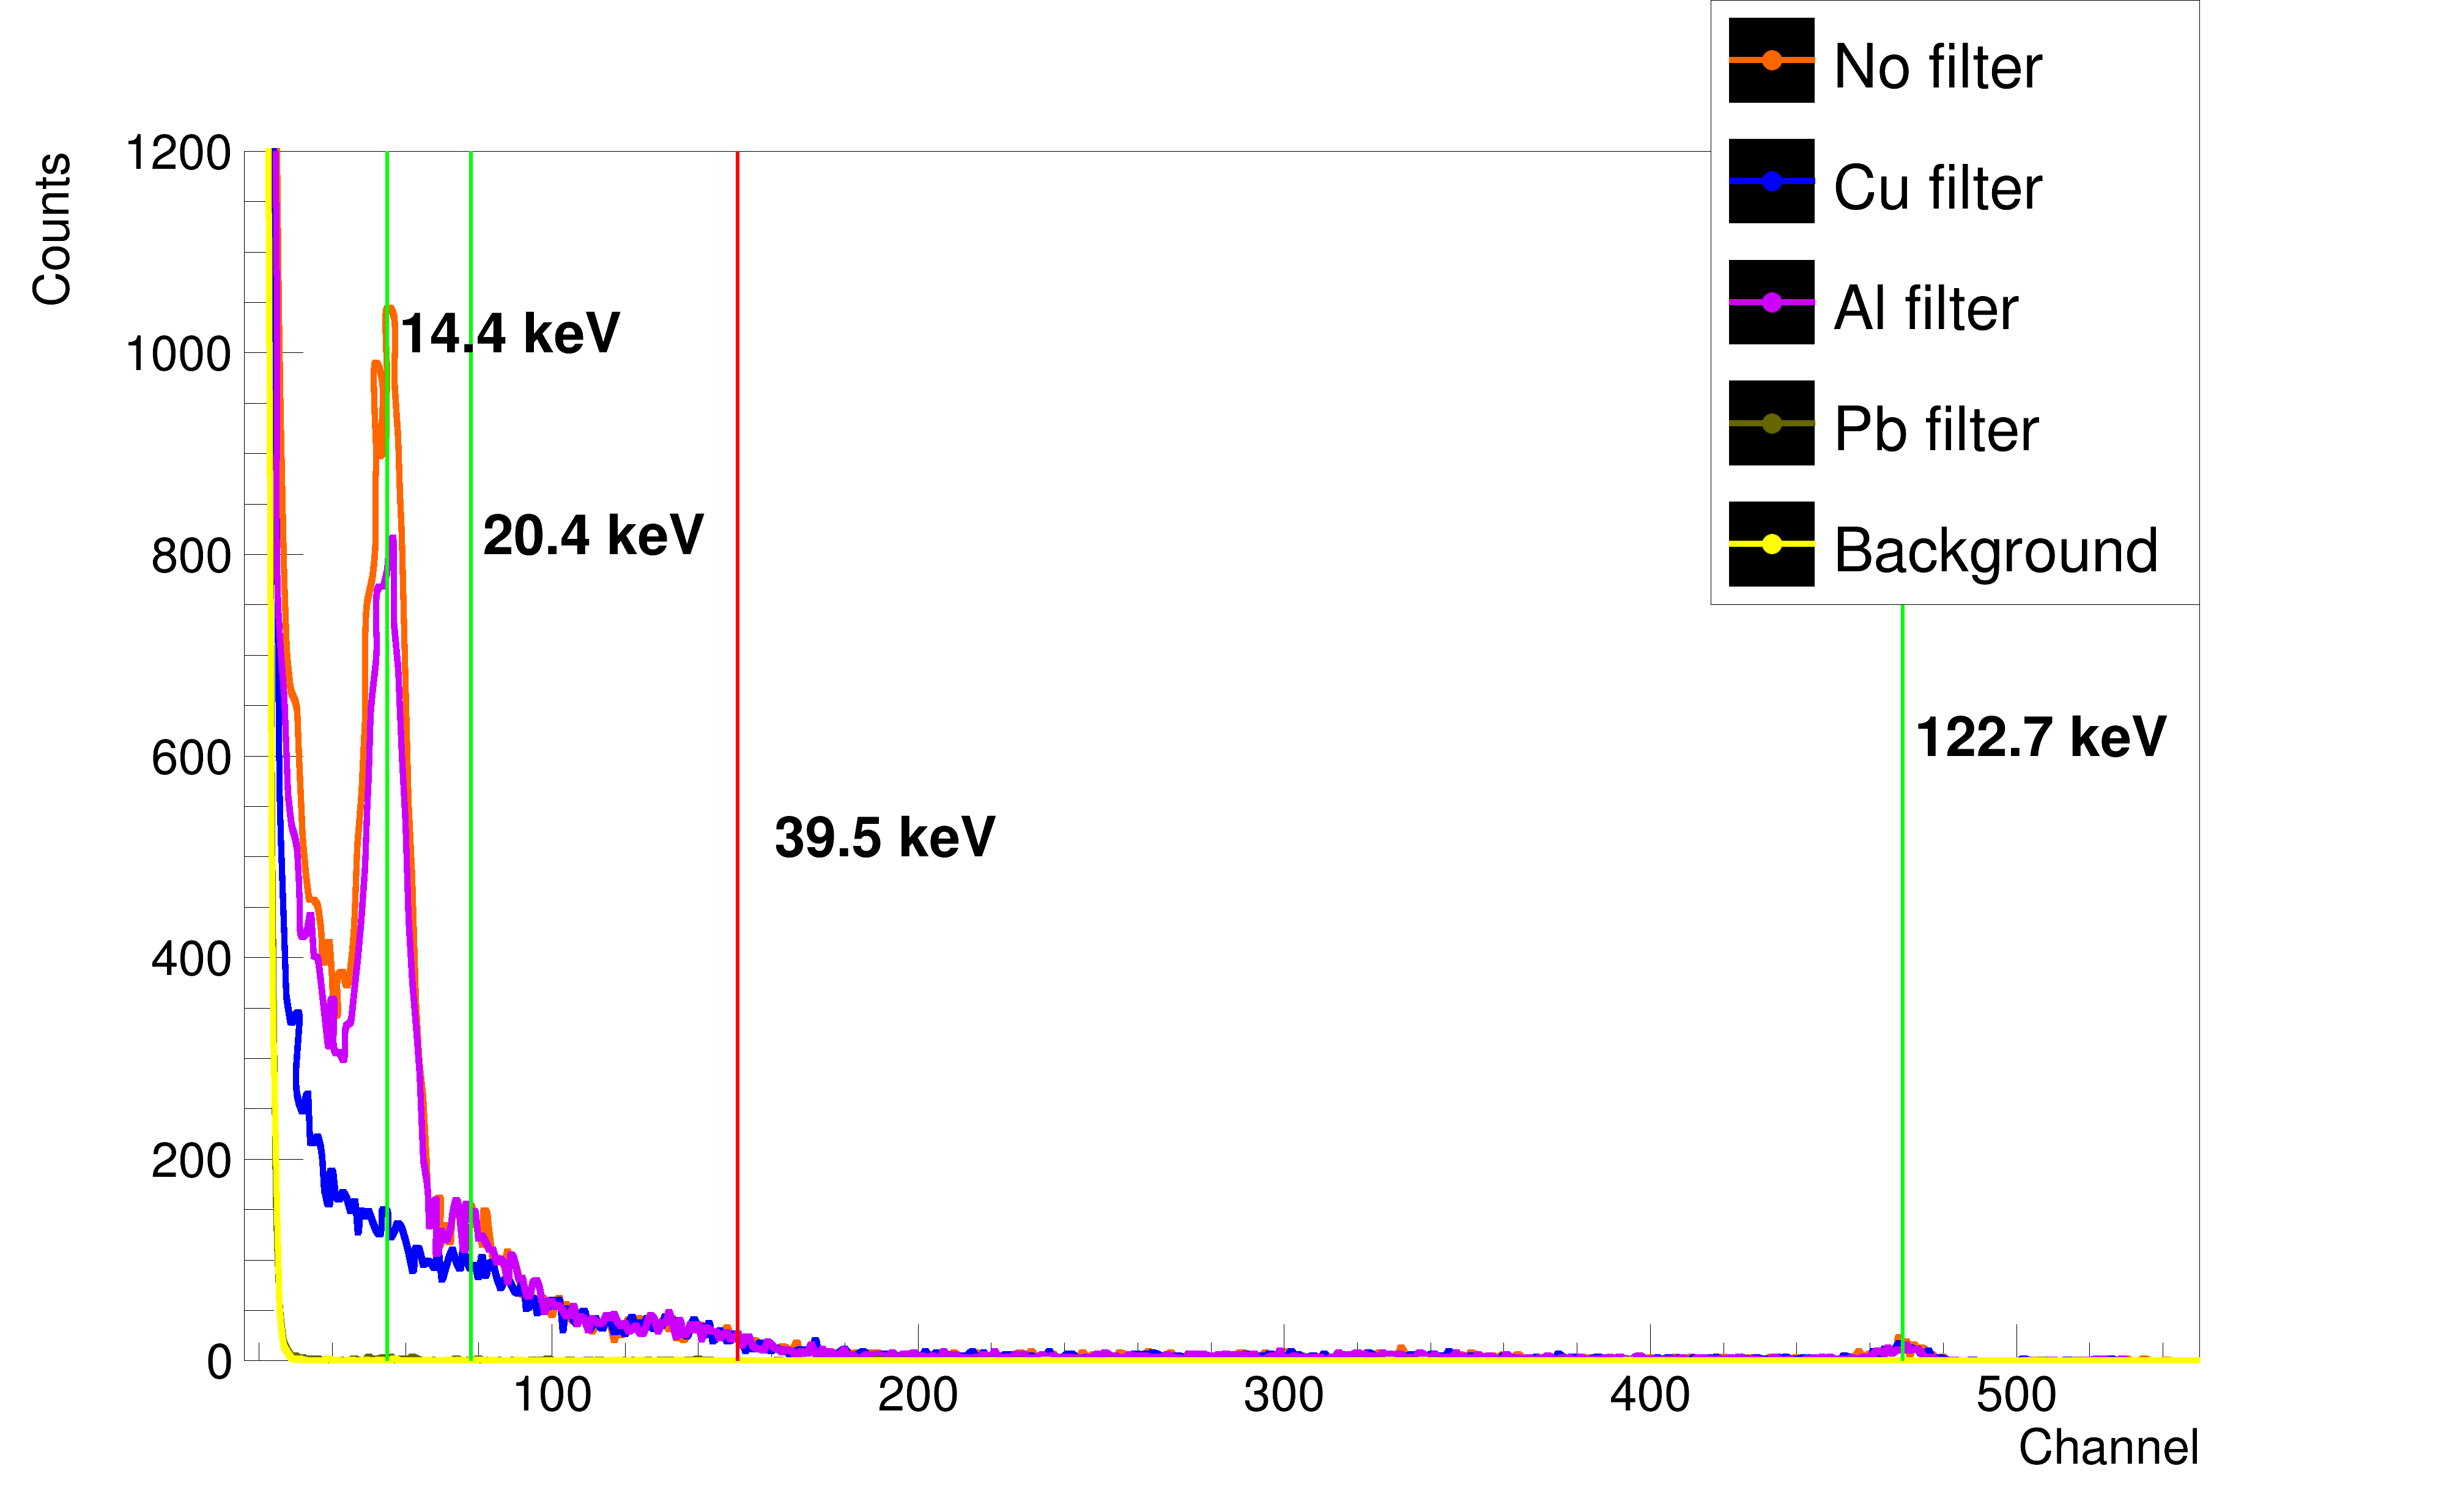
\includegraphics[scale=0.125, angle = 0]{./pictures/BPW34GammaTest.png}
  \caption{BPW34 spectra with founded energy peaks (green lines) and estimated Compton edge (red line).}
 \label{BPW34 spectra}
 
\end{figure}

The measured spectra of BPW34 is very similar to the previous one, however the peak's heights are approximately 25 times lower.

It is surprising that this cheap photodiode is capable of capturing gamma rays with sufficient energy resolution.
\subsection{OPF430 test}
OPF430 was operated at 20 V. There was a problem with the very low detection efficiency, so the source had to be put into the shielding box right before the photodiode.

\begin{figure}[H]
 \centering
 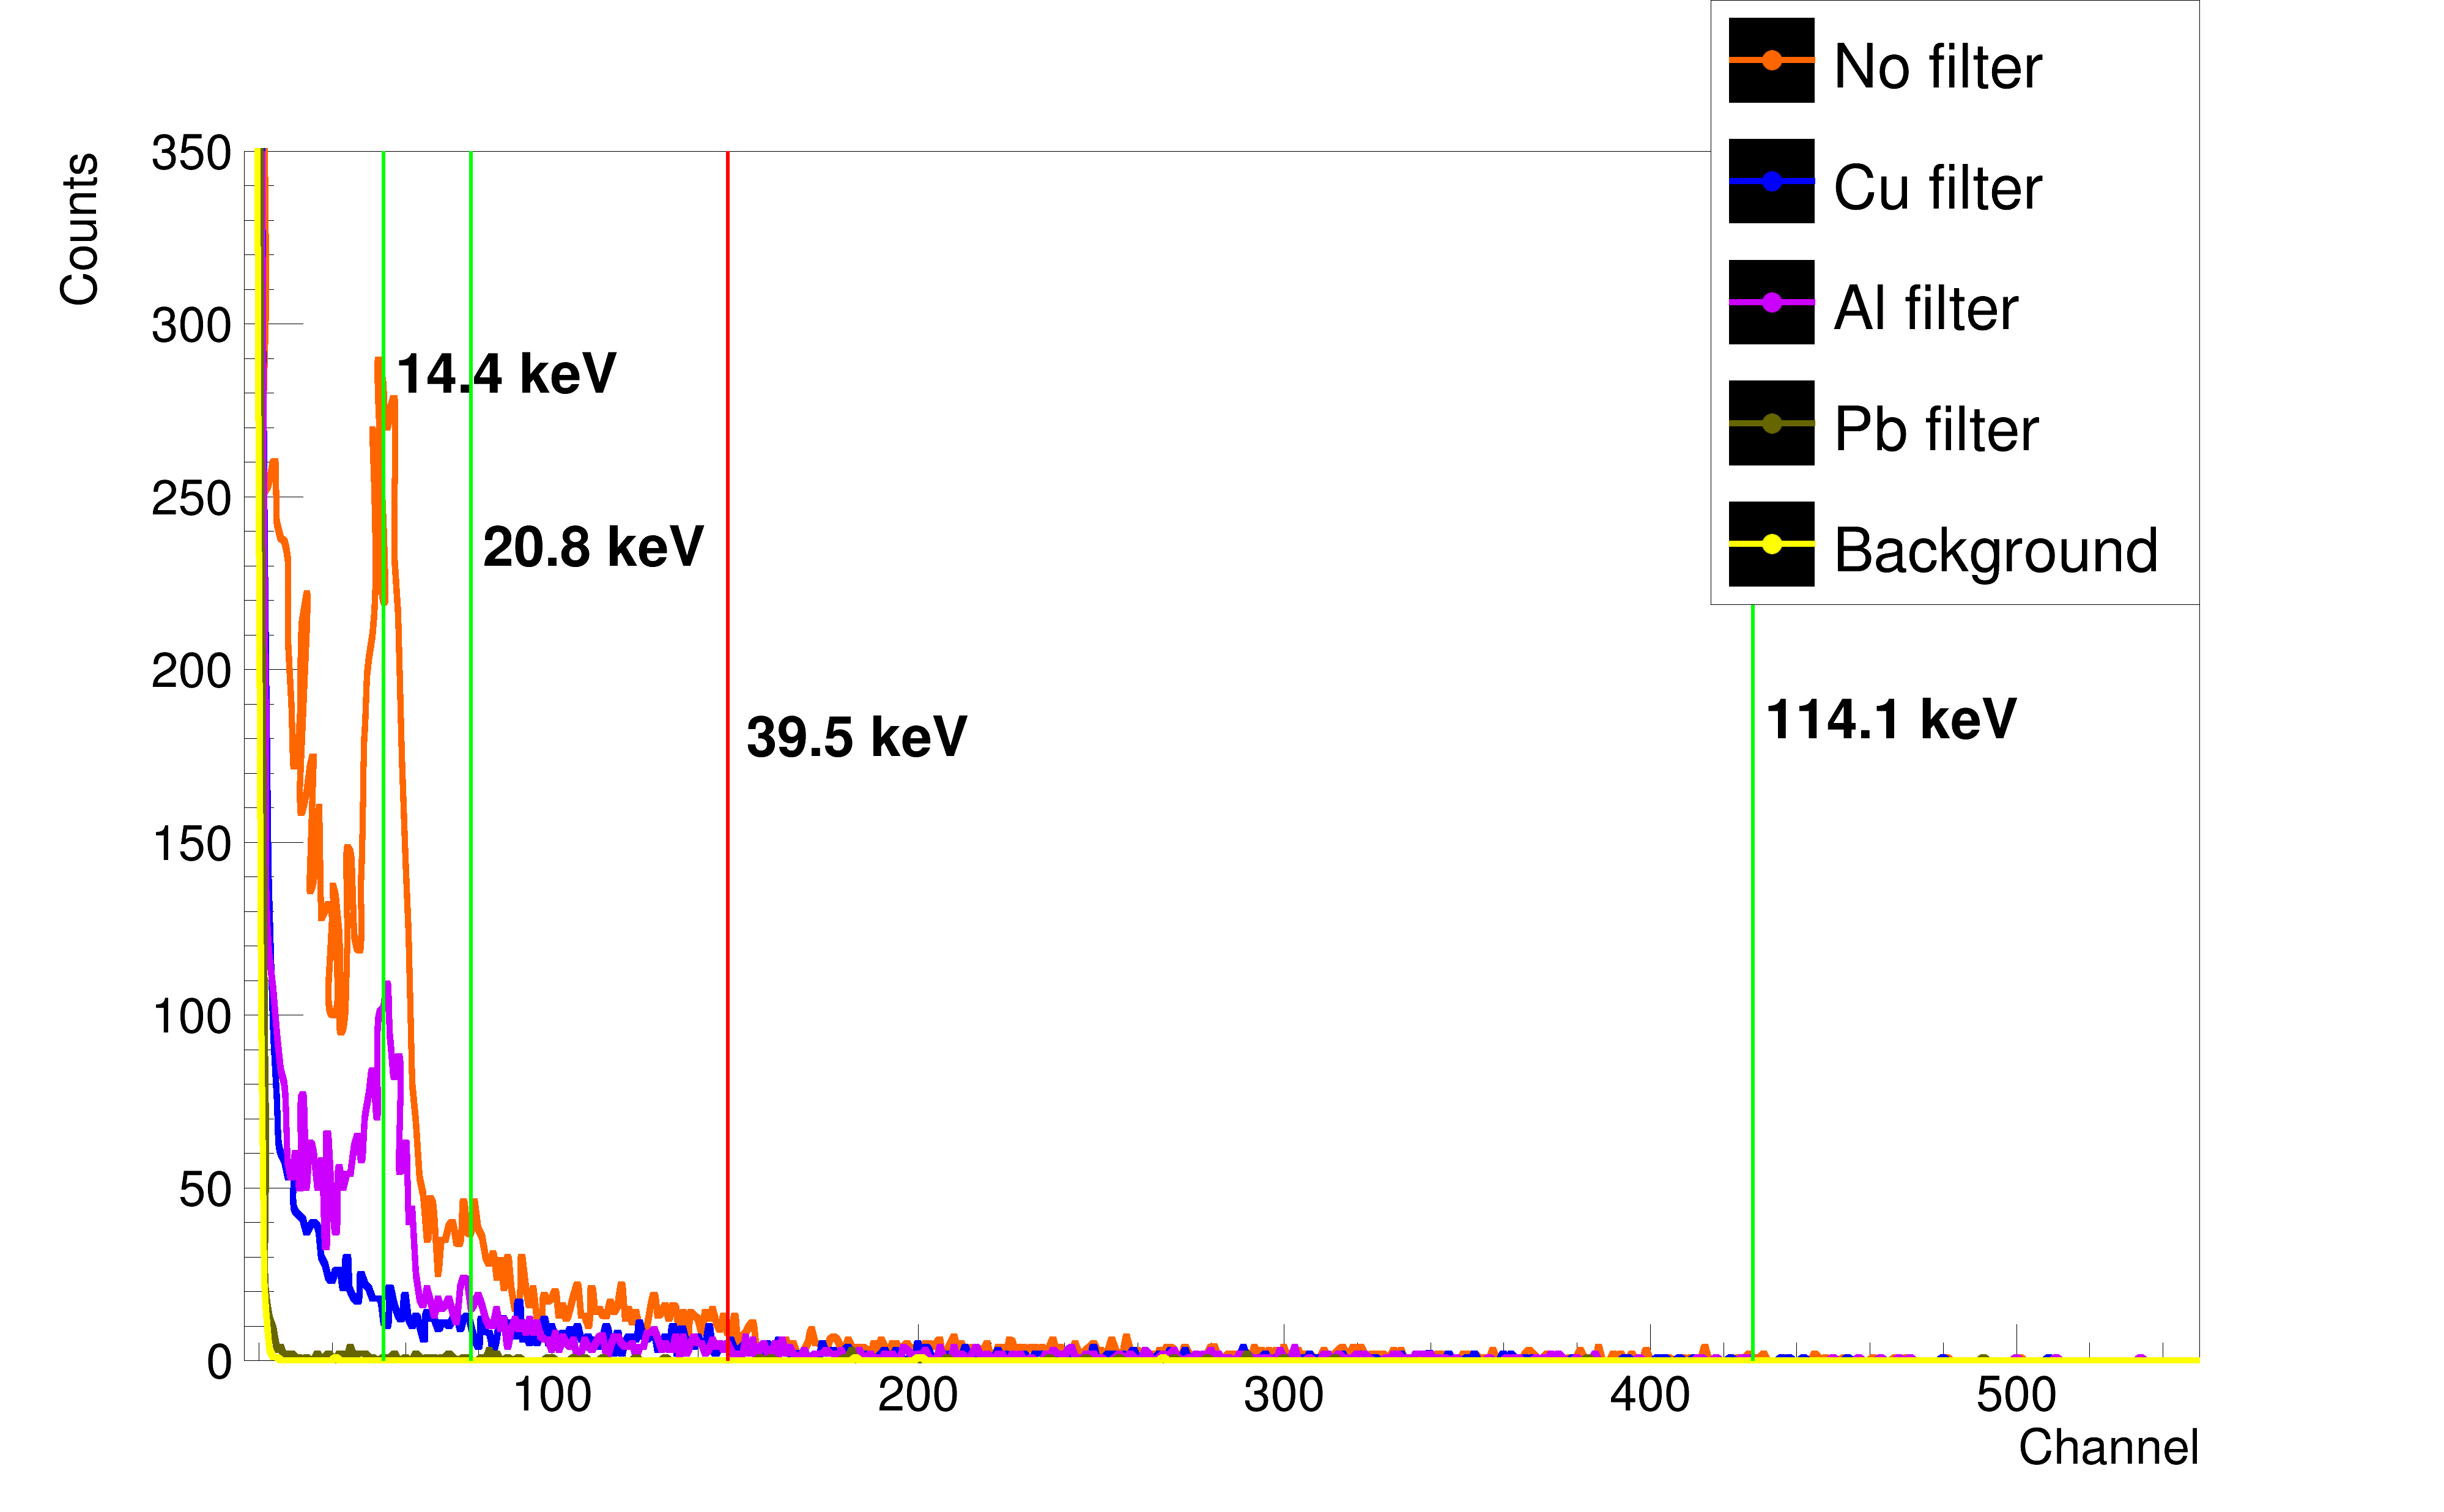
\includegraphics[scale=0.125, angle = 0]{./pictures/OPF430GammaTest.png}
 \caption{OPF430 spectra with founded energy peaks (green lines) and estimated Compton edge (red line).}
 \label{OPF430 spectra}
 
\end{figure}

It can be seen that the count rates are still much lower that they were measured at previous photodiodes. This is probably due to the fact, that the surface of detector is very small.
The conclusion is that OPF430 is capable of capturing the low-energy gamma rays, however, the efficiency is so bad that it makes it unusable for any real gamma spectroscopy application. 
